\chead{\textit{Results}}  				
\section{Results}
\label{sec:res}

The following chapter presents the results of this thesis. First, a case study system is presented that is used as a reference example to calculate both the centralized problem and the decentralized problem. Following this, the results of both approaches are compared against each other. Next, the convergence of the decentralized algorithm is analyzed and several issues are presented that influence the convergence rate of the algorithm.

\subsection{Case Study System}
\label{sec:res:tns}

The following section describes the \gls{tns} that is used as a case study system to examine the decentralized optimal power flow implementation. Hereby, the system is rather simple to better grasp the findings. As mentioned in section \ref{sec:app:implementation}, the source code can be easily extended by more detailed case study systems. The \gls{tns} consists of three nodes. At each of them, a different set of generators and storages is located. Each node has a different two period demand vector. The nodes are connected by a total of three transmission lines. Thus, every node has two neighbors. All network elements must meet the requirements described in section (\ref{sec:app:mod-framework}). The network layout and the corresponding parameters of the elements are shown in figure (\ref{fig:tns}).

\begin{figure}[h]
	\centering
	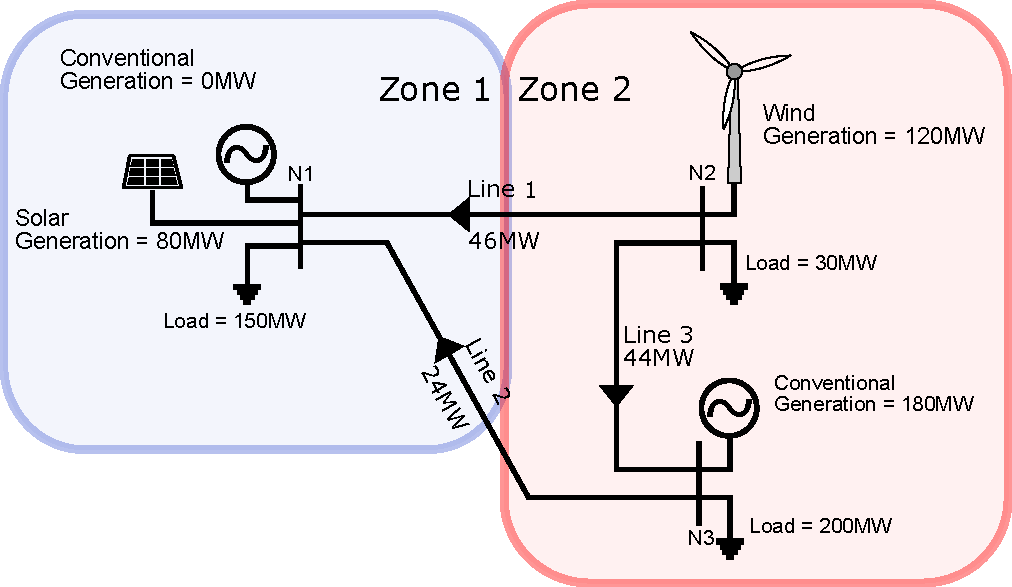
\includegraphics[width=\textwidth]{three-node-system.png}
	\caption{Exemplary Three Node System}
	\label{fig:tns}
\end{figure}

There is a total of four generators in the system. The name of the generators refer to real life power plants. For example, the coal generator at node 3 (N3) has the largest production capacity and is more expensive than the photovoltaic and wind generator. The gas generator on the other hand, has the highest marginal costs in the system to account for a generator that is only used to cover peak loads. The marginal costs for the renewable generators are not set to zero because this would violate the penalty terms. Thus, they are set to 3 and 4 respectively. All generator specific parameters are listed in table \ref{tab:res:param-gen}.

\begin{table}[ht]
    \centering
    \begin{tabular}{lrr}
        Generators $\set{G}$ & $mc$ [\euro/MWh] & $\overline{p}$ [MW] \\ \toprule
        PV & 3 & 80 \\
        Wind & 4 & 120 \\
        Coal & 30 & 300 \\
        Gas & 50 & 120 \\
        \bottomrule
    \end{tabular}
    \caption{Generator parameters for Three Node System} \label{tab:res:param-gen}
\end{table}

In addition to the generators, there is one storage in the \gls{tns} that is located at node 1. This network element has the cheapest marginal costs to ensure that the storage is favored in all dispatch decisions. The parameters of the storage are shown in table \ref{tab:res:param-stor}.

 \begin{table}[ht]
    \centering
    \begin{tabular}{lrrr}
        Storages $\set{S}$ & $mc$ [\euro/MWh] & $\overline{p}$ [MW] & $\overline{e}$ [MWh] \\ \toprule
        Battery & 1 & 10 & 20 \\
        \bottomrule
    \end{tabular}
    \caption{Storage parameters for Three Node System} \label{tab:res:param-stor}
\end{table}

Lastly, the capacities of the transmission lines are set to values so that a congestion on either one line is most certain. All relevant parameters of all three transmission lines can be found in table \ref{tab:res:param-line}.

 \begin{table}[ht]
    \centering
    \begin{tabular}{lrr}
        Transmission Lines $\set{L}$ & $f$ [MWh] & $S$ [1/$\Omega$] \\ \toprule
        Line 1 & 20 & 1 \\
        Line 2 & 45 & 1 \\
        Line 3 & 70 & 2 \\
        \bottomrule
    \end{tabular}
    \caption{Transmission line parameters for Three Node System} \label{tab:res:param-line}
\end{table}